% Graphic for TeX using PGF
% Title: S:\Senior Project\seniorProject2-2020-21-Docs\figs\dia\systemOperationFlowchart.dia
% Creator: Dia v0.97.2
% CreationDate: Tue Dec 01 10:06:16 2020
% For: Jason Braker
% \usepackage{tikz}
% The following commands are not supported in PSTricks at present
% We define them conditionally, so when they are implemented,
% this pgf file will use them.
\ifx\du\undefined
  \newlength{\du}
\fi
\setlength{\du}{15\unitlength}
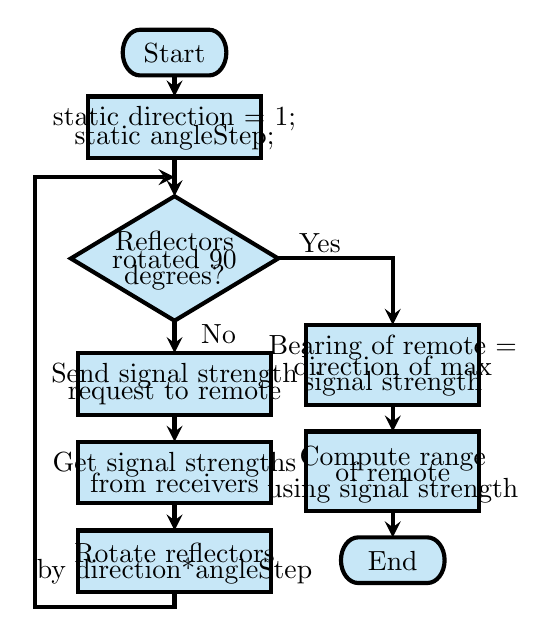
\begin{tikzpicture}[scale=0.55]
\pgftransformxscale{1.000000}
\pgftransformyscale{-1.000000}
\definecolor{dialinecolor}{rgb}{0.000000, 0.000000, 0.000000}
\pgfsetstrokecolor{dialinecolor}
\definecolor{dialinecolor}{rgb}{1.000000, 1.000000, 1.000000}
\pgfsetfillcolor{dialinecolor}
\pgfsetlinewidth{0.100000\du}
\pgfsetdash{}{0pt}
\pgfsetdash{}{0pt}
\pgfsetbuttcap
\pgfsetmiterjoin
\pgfsetlinewidth{0.100000\du}
\pgfsetbuttcap
\pgfsetmiterjoin
\pgfsetdash{}{0pt}
\definecolor{dialinecolor}{rgb}{0.780392, 0.905882, 0.968627}
\pgfsetfillcolor{dialinecolor}
\pgfpathmoveto{\pgfpoint{23.245553\du}{0.476720\du}}
\pgfpathlineto{\pgfpoint{26.271803\du}{0.476720\du}}
\pgfpathcurveto{\pgfpoint{26.689641\du}{0.476720\du}}{\pgfpoint{27.028366\du}{0.924435\du}}{\pgfpoint{27.028366\du}{1.476720\du}}
\pgfpathcurveto{\pgfpoint{27.028366\du}{2.029005\du}}{\pgfpoint{26.689641\du}{2.476720\du}}{\pgfpoint{26.271803\du}{2.476720\du}}
\pgfpathlineto{\pgfpoint{23.245553\du}{2.476720\du}}
\pgfpathcurveto{\pgfpoint{22.827715\du}{2.476720\du}}{\pgfpoint{22.488991\du}{2.029005\du}}{\pgfpoint{22.488991\du}{1.476720\du}}
\pgfpathcurveto{\pgfpoint{22.488991\du}{0.924435\du}}{\pgfpoint{22.827715\du}{0.476720\du}}{\pgfpoint{23.245553\du}{0.476720\du}}
\pgfusepath{fill}
\definecolor{dialinecolor}{rgb}{0.000000, 0.000000, 0.000000}
\pgfsetstrokecolor{dialinecolor}
\pgfpathmoveto{\pgfpoint{23.245553\du}{0.476720\du}}
\pgfpathlineto{\pgfpoint{26.271803\du}{0.476720\du}}
\pgfpathcurveto{\pgfpoint{26.689641\du}{0.476720\du}}{\pgfpoint{27.028366\du}{0.924435\du}}{\pgfpoint{27.028366\du}{1.476720\du}}
\pgfpathcurveto{\pgfpoint{27.028366\du}{2.029005\du}}{\pgfpoint{26.689641\du}{2.476720\du}}{\pgfpoint{26.271803\du}{2.476720\du}}
\pgfpathlineto{\pgfpoint{23.245553\du}{2.476720\du}}
\pgfpathcurveto{\pgfpoint{22.827715\du}{2.476720\du}}{\pgfpoint{22.488991\du}{2.029005\du}}{\pgfpoint{22.488991\du}{1.476720\du}}
\pgfpathcurveto{\pgfpoint{22.488991\du}{0.924435\du}}{\pgfpoint{22.827715\du}{0.476720\du}}{\pgfpoint{23.245553\du}{0.476720\du}}
\pgfusepath{stroke}
% setfont left to latex
\definecolor{dialinecolor}{rgb}{0.000000, 0.000000, 0.000000}
\pgfsetstrokecolor{dialinecolor}
\node at (24.758678\du,1.516720\du){Start};
\pgfsetlinewidth{0.100000\du}
\pgfsetdash{}{0pt}
\pgfsetdash{}{0pt}
\pgfsetbuttcap
{
\definecolor{dialinecolor}{rgb}{0.000000, 0.000000, 0.000000}
\pgfsetfillcolor{dialinecolor}
% was here!!!
\pgfsetarrowsend{stealth}
\definecolor{dialinecolor}{rgb}{0.000000, 0.000000, 0.000000}
\pgfsetstrokecolor{dialinecolor}
\draw (24.758678\du,13.254938\du)--(24.758678\du,14.638000\du);
}
\pgfsetlinewidth{0.100000\du}
\pgfsetdash{}{0pt}
\pgfsetdash{}{0pt}
\pgfsetbuttcap
{
\definecolor{dialinecolor}{rgb}{0.000000, 0.000000, 0.000000}
\pgfsetfillcolor{dialinecolor}
% was here!!!
\pgfsetarrowsend{stealth}
\definecolor{dialinecolor}{rgb}{0.000000, 0.000000, 0.000000}
\pgfsetstrokecolor{dialinecolor}
\draw (24.758678\du,6.097900\du)--(24.758678\du,7.767002\du);
}
\pgfsetlinewidth{0.100000\du}
\pgfsetdash{}{0pt}
\pgfsetdash{}{0pt}
\pgfsetmiterjoin
\pgfsetbuttcap
{
\definecolor{dialinecolor}{rgb}{0.000000, 0.000000, 0.000000}
\pgfsetfillcolor{dialinecolor}
% was here!!!
\pgfsetarrowsend{stealth}
{\pgfsetcornersarced{\pgfpoint{0.000000\du}{0.000000\du}}\definecolor{dialinecolor}{rgb}{0.000000, 0.000000, 0.000000}
\pgfsetstrokecolor{dialinecolor}
\draw (24.758678\du,25.106700\du)--(24.758678\du,25.775000\du)--(18.662000\du,25.775000\du)--(18.662000\du,6.932451\du)--(24.758678\du,6.932451\du);
}}
\pgfsetlinewidth{0.100000\du}
\pgfsetdash{}{0pt}
\pgfsetdash{}{0pt}
\pgfsetmiterjoin
\pgfsetbuttcap
{
\definecolor{dialinecolor}{rgb}{0.000000, 0.000000, 0.000000}
\pgfsetfillcolor{dialinecolor}
% was here!!!
\pgfsetarrowsend{stealth}
{\pgfsetcornersarced{\pgfpoint{0.000000\du}{0.000000\du}}\definecolor{dialinecolor}{rgb}{0.000000, 0.000000, 0.000000}
\pgfsetstrokecolor{dialinecolor}
\draw (29.260647\du,10.510970\du)--(29.260647\du,10.475000\du)--(34.317800\du,10.475000\du)--(34.317800\du,13.401800\du);
}}
% setfont left to latex
\definecolor{dialinecolor}{rgb}{0.000000, 0.000000, 0.000000}
\pgfsetstrokecolor{dialinecolor}
\node[anchor=west] at (29.716400\du,9.806400\du){Yes};
% setfont left to latex
\definecolor{dialinecolor}{rgb}{0.000000, 0.000000, 0.000000}
\pgfsetstrokecolor{dialinecolor}
\node[anchor=west] at (25.433800\du,13.804600\du){No};
\definecolor{dialinecolor}{rgb}{0.780392, 0.905882, 0.968627}
\pgfsetfillcolor{dialinecolor}
\fill (20.519144\du,18.522300\du)--(20.519144\du,21.222300\du)--(28.998212\du,21.222300\du)--(28.998212\du,18.522300\du)--cycle;
\pgfsetlinewidth{0.100000\du}
\pgfsetdash{}{0pt}
\pgfsetdash{}{0pt}
\pgfsetmiterjoin
\definecolor{dialinecolor}{rgb}{0.000000, 0.000000, 0.000000}
\pgfsetstrokecolor{dialinecolor}
\draw (20.519144\du,18.522300\du)--(20.519144\du,21.222300\du)--(28.998212\du,21.222300\du)--(28.998212\du,18.522300\du)--cycle;
% setfont left to latex
\definecolor{dialinecolor}{rgb}{0.000000, 0.000000, 0.000000}
\pgfsetstrokecolor{dialinecolor}
\node at (24.758678\du,19.512300\du){Get signal strengths};
% setfont left to latex
\definecolor{dialinecolor}{rgb}{0.000000, 0.000000, 0.000000}
\pgfsetstrokecolor{dialinecolor}
\node at (24.758678\du,20.312300\du){from receivers};
\definecolor{dialinecolor}{rgb}{0.780392, 0.905882, 0.968627}
\pgfsetfillcolor{dialinecolor}
\fill (24.758678\du,7.767002\du)--(29.299535\du,10.494358\du)--(24.758678\du,13.221715\du)--(20.217821\du,10.494358\du)--cycle;
\pgfsetlinewidth{0.100000\du}
\pgfsetdash{}{0pt}
\pgfsetdash{}{0pt}
\pgfsetmiterjoin
\definecolor{dialinecolor}{rgb}{0.000000, 0.000000, 0.000000}
\pgfsetstrokecolor{dialinecolor}
\draw (24.758678\du,7.767002\du)--(29.299535\du,10.494358\du)--(24.758678\du,13.221715\du)--(20.217821\du,10.494358\du)--cycle;
% setfont left to latex
\definecolor{dialinecolor}{rgb}{0.000000, 0.000000, 0.000000}
\pgfsetstrokecolor{dialinecolor}
\node at (24.758678\du,9.734358\du){Reflectors};
% setfont left to latex
\definecolor{dialinecolor}{rgb}{0.000000, 0.000000, 0.000000}
\pgfsetstrokecolor{dialinecolor}
\node at (24.758678\du,10.534358\du){rotated 90};
% setfont left to latex
\definecolor{dialinecolor}{rgb}{0.000000, 0.000000, 0.000000}
\pgfsetstrokecolor{dialinecolor}
\node at (24.758678\du,11.334358\du){degrees?};
\definecolor{dialinecolor}{rgb}{0.780392, 0.905882, 0.968627}
\pgfsetfillcolor{dialinecolor}
\fill (30.525300\du,13.401800\du)--(30.525300\du,16.901800\du)--(38.110300\du,16.901800\du)--(38.110300\du,13.401800\du)--cycle;
\pgfsetlinewidth{0.100000\du}
\pgfsetdash{}{0pt}
\pgfsetdash{}{0pt}
\pgfsetmiterjoin
\definecolor{dialinecolor}{rgb}{0.000000, 0.000000, 0.000000}
\pgfsetstrokecolor{dialinecolor}
\draw (30.525300\du,13.401800\du)--(30.525300\du,16.901800\du)--(38.110300\du,16.901800\du)--(38.110300\du,13.401800\du)--cycle;
% setfont left to latex
\definecolor{dialinecolor}{rgb}{0.000000, 0.000000, 0.000000}
\pgfsetstrokecolor{dialinecolor}
\node at (34.317800\du,14.391800\du){Bearing of remote =};
% setfont left to latex
\definecolor{dialinecolor}{rgb}{0.000000, 0.000000, 0.000000}
\pgfsetstrokecolor{dialinecolor}
\node at (34.317800\du,15.191800\du){direction of max};
% setfont left to latex
\definecolor{dialinecolor}{rgb}{0.000000, 0.000000, 0.000000}
\pgfsetstrokecolor{dialinecolor}
\node at (34.317800\du,15.991800\du){signal strength};
\definecolor{dialinecolor}{rgb}{0.780392, 0.905882, 0.968627}
\pgfsetfillcolor{dialinecolor}
\fill (30.525300\du,18.072900\du)--(30.525300\du,21.572900\du)--(38.110300\du,21.572900\du)--(38.110300\du,18.072900\du)--cycle;
\pgfsetlinewidth{0.100000\du}
\pgfsetdash{}{0pt}
\pgfsetdash{}{0pt}
\pgfsetmiterjoin
\definecolor{dialinecolor}{rgb}{0.000000, 0.000000, 0.000000}
\pgfsetstrokecolor{dialinecolor}
\draw (30.525300\du,18.072900\du)--(30.525300\du,21.572900\du)--(38.110300\du,21.572900\du)--(38.110300\du,18.072900\du)--cycle;
% setfont left to latex
\definecolor{dialinecolor}{rgb}{0.000000, 0.000000, 0.000000}
\pgfsetstrokecolor{dialinecolor}
\node at (34.317800\du,19.262900\du){Compute range};
% setfont left to latex
\definecolor{dialinecolor}{rgb}{0.000000, 0.000000, 0.000000}
\pgfsetstrokecolor{dialinecolor}
\node at (34.317800\du,19.862900\du){of remote};
% setfont left to latex
\definecolor{dialinecolor}{rgb}{0.000000, 0.000000, 0.000000}
\pgfsetstrokecolor{dialinecolor}
\node at (34.317800\du,20.662900\du){using signal strength};
\pgfsetlinewidth{0.100000\du}
\pgfsetdash{}{0pt}
\pgfsetdash{}{0pt}
\pgfsetbuttcap
{
\definecolor{dialinecolor}{rgb}{0.000000, 0.000000, 0.000000}
\pgfsetfillcolor{dialinecolor}
% was here!!!
\pgfsetarrowsend{stealth}
\definecolor{dialinecolor}{rgb}{0.000000, 0.000000, 0.000000}
\pgfsetstrokecolor{dialinecolor}
\draw (24.758678\du,17.338000\du)--(24.758678\du,18.522300\du);
}
\pgfsetlinewidth{0.100000\du}
\pgfsetdash{}{0pt}
\pgfsetdash{}{0pt}
\pgfsetbuttcap
{
\definecolor{dialinecolor}{rgb}{0.000000, 0.000000, 0.000000}
\pgfsetfillcolor{dialinecolor}
% was here!!!
\pgfsetarrowsend{stealth}
\definecolor{dialinecolor}{rgb}{0.000000, 0.000000, 0.000000}
\pgfsetstrokecolor{dialinecolor}
\draw (24.758678\du,21.222300\du)--(24.758678\du,22.406700\du);
}
\pgfsetlinewidth{0.100000\du}
\pgfsetdash{}{0pt}
\pgfsetdash{}{0pt}
\pgfsetbuttcap
{
\definecolor{dialinecolor}{rgb}{0.000000, 0.000000, 0.000000}
\pgfsetfillcolor{dialinecolor}
% was here!!!
\pgfsetarrowsend{stealth}
\definecolor{dialinecolor}{rgb}{0.000000, 0.000000, 0.000000}
\pgfsetstrokecolor{dialinecolor}
\draw (34.317800\du,16.901800\du)--(34.317800\du,18.072900\du);
}
\pgfsetlinewidth{0.100000\du}
\pgfsetdash{}{0pt}
\pgfsetdash{}{0pt}
\pgfsetbuttcap
{
\definecolor{dialinecolor}{rgb}{0.000000, 0.000000, 0.000000}
\pgfsetfillcolor{dialinecolor}
% was here!!!
\pgfsetarrowsend{stealth}
\definecolor{dialinecolor}{rgb}{0.000000, 0.000000, 0.000000}
\pgfsetstrokecolor{dialinecolor}
\draw (34.317800\du,21.572900\du)--(34.317800\du,22.709900\du);
}
\definecolor{dialinecolor}{rgb}{0.780392, 0.905882, 0.968627}
\pgfsetfillcolor{dialinecolor}
\fill (20.519144\du,14.638000\du)--(20.519144\du,17.338000\du)--(28.998212\du,17.338000\du)--(28.998212\du,14.638000\du)--cycle;
\pgfsetlinewidth{0.100000\du}
\pgfsetdash{}{0pt}
\pgfsetdash{}{0pt}
\pgfsetmiterjoin
\definecolor{dialinecolor}{rgb}{0.000000, 0.000000, 0.000000}
\pgfsetstrokecolor{dialinecolor}
\draw (20.519144\du,14.638000\du)--(20.519144\du,17.338000\du)--(28.998212\du,17.338000\du)--(28.998212\du,14.638000\du)--cycle;
% setfont left to latex
\definecolor{dialinecolor}{rgb}{0.000000, 0.000000, 0.000000}
\pgfsetstrokecolor{dialinecolor}
\node at (24.758678\du,15.628000\du){Send signal strength};
% setfont left to latex
\definecolor{dialinecolor}{rgb}{0.000000, 0.000000, 0.000000}
\pgfsetstrokecolor{dialinecolor}
\node at (24.758678\du,16.428000\du){request to remote};
\definecolor{dialinecolor}{rgb}{0.780392, 0.905882, 0.968627}
\pgfsetfillcolor{dialinecolor}
\fill (20.519144\du,22.406700\du)--(20.519144\du,25.106700\du)--(28.998212\du,25.106700\du)--(28.998212\du,22.406700\du)--cycle;
\pgfsetlinewidth{0.100000\du}
\pgfsetdash{}{0pt}
\pgfsetdash{}{0pt}
\pgfsetmiterjoin
\definecolor{dialinecolor}{rgb}{0.000000, 0.000000, 0.000000}
\pgfsetstrokecolor{dialinecolor}
\draw (20.519144\du,22.406700\du)--(20.519144\du,25.106700\du)--(28.998212\du,25.106700\du)--(28.998212\du,22.406700\du)--cycle;
% setfont left to latex
\definecolor{dialinecolor}{rgb}{0.000000, 0.000000, 0.000000}
\pgfsetstrokecolor{dialinecolor}
\node at (24.758678\du,23.396700\du){Rotate reflectors};
% setfont left to latex
\definecolor{dialinecolor}{rgb}{0.000000, 0.000000, 0.000000}
\pgfsetstrokecolor{dialinecolor}
\node at (24.758678\du,24.196700\du){by direction*angleStep};
\pgfsetlinewidth{0.100000\du}
\pgfsetdash{}{0pt}
\pgfsetdash{}{0pt}
\pgfsetbuttcap
\pgfsetmiterjoin
\pgfsetlinewidth{0.100000\du}
\pgfsetbuttcap
\pgfsetmiterjoin
\pgfsetdash{}{0pt}
\definecolor{dialinecolor}{rgb}{0.780392, 0.905882, 0.968627}
\pgfsetfillcolor{dialinecolor}
\pgfpathmoveto{\pgfpoint{32.804675\du}{22.709900\du}}
\pgfpathlineto{\pgfpoint{35.830925\du}{22.709900\du}}
\pgfpathcurveto{\pgfpoint{36.248763\du}{22.709900\du}}{\pgfpoint{36.587488\du}{23.157615\du}}{\pgfpoint{36.587488\du}{23.709900\du}}
\pgfpathcurveto{\pgfpoint{36.587488\du}{24.262185\du}}{\pgfpoint{36.248763\du}{24.709900\du}}{\pgfpoint{35.830925\du}{24.709900\du}}
\pgfpathlineto{\pgfpoint{32.804675\du}{24.709900\du}}
\pgfpathcurveto{\pgfpoint{32.386837\du}{24.709900\du}}{\pgfpoint{32.048113\du}{24.262185\du}}{\pgfpoint{32.048113\du}{23.709900\du}}
\pgfpathcurveto{\pgfpoint{32.048113\du}{23.157615\du}}{\pgfpoint{32.386837\du}{22.709900\du}}{\pgfpoint{32.804675\du}{22.709900\du}}
\pgfusepath{fill}
\definecolor{dialinecolor}{rgb}{0.000000, 0.000000, 0.000000}
\pgfsetstrokecolor{dialinecolor}
\pgfpathmoveto{\pgfpoint{32.804675\du}{22.709900\du}}
\pgfpathlineto{\pgfpoint{35.830925\du}{22.709900\du}}
\pgfpathcurveto{\pgfpoint{36.248763\du}{22.709900\du}}{\pgfpoint{36.587488\du}{23.157615\du}}{\pgfpoint{36.587488\du}{23.709900\du}}
\pgfpathcurveto{\pgfpoint{36.587488\du}{24.262185\du}}{\pgfpoint{36.248763\du}{24.709900\du}}{\pgfpoint{35.830925\du}{24.709900\du}}
\pgfpathlineto{\pgfpoint{32.804675\du}{24.709900\du}}
\pgfpathcurveto{\pgfpoint{32.386837\du}{24.709900\du}}{\pgfpoint{32.048113\du}{24.262185\du}}{\pgfpoint{32.048113\du}{23.709900\du}}
\pgfpathcurveto{\pgfpoint{32.048113\du}{23.157615\du}}{\pgfpoint{32.386837\du}{22.709900\du}}{\pgfpoint{32.804675\du}{22.709900\du}}
\pgfusepath{stroke}
% setfont left to latex
\definecolor{dialinecolor}{rgb}{0.000000, 0.000000, 0.000000}
\pgfsetstrokecolor{dialinecolor}
\node at (34.317800\du,23.749900\du){End};
\definecolor{dialinecolor}{rgb}{0.780392, 0.905882, 0.968627}
\pgfsetfillcolor{dialinecolor}
\fill (20.966178\du,3.397900\du)--(20.966178\du,6.097900\du)--(28.551178\du,6.097900\du)--(28.551178\du,3.397900\du)--cycle;
\pgfsetlinewidth{0.100000\du}
\pgfsetdash{}{0pt}
\pgfsetdash{}{0pt}
\pgfsetmiterjoin
\definecolor{dialinecolor}{rgb}{0.000000, 0.000000, 0.000000}
\pgfsetstrokecolor{dialinecolor}
\draw (20.966178\du,3.397900\du)--(20.966178\du,6.097900\du)--(28.551178\du,6.097900\du)--(28.551178\du,3.397900\du)--cycle;
% setfont left to latex
\definecolor{dialinecolor}{rgb}{0.000000, 0.000000, 0.000000}
\pgfsetstrokecolor{dialinecolor}
\node at (24.758678\du,4.387900\du){static direction = 1;};
% setfont left to latex
\definecolor{dialinecolor}{rgb}{0.000000, 0.000000, 0.000000}
\pgfsetstrokecolor{dialinecolor}
\node at (24.758678\du,5.187900\du){static angleStep;};
\pgfsetlinewidth{0.100000\du}
\pgfsetdash{}{0pt}
\pgfsetdash{}{0pt}
\pgfsetbuttcap
{
\definecolor{dialinecolor}{rgb}{0.000000, 0.000000, 0.000000}
\pgfsetfillcolor{dialinecolor}
% was here!!!
\pgfsetarrowsend{stealth}
\definecolor{dialinecolor}{rgb}{0.000000, 0.000000, 0.000000}
\pgfsetstrokecolor{dialinecolor}
\draw (24.758678\du,2.476720\du)--(24.758678\du,3.397900\du);
}
\end{tikzpicture}
